\subsubsection*{Problem definition}

The first example for transverse isotropic ellasticity is the twodimensional simplification of the tension of a quadratic plate under plane strain conditions according to Schr\"oder \cite{Schroeder:1996} and Kohlmeier \cite{Kohlmeier:2006}. Within this context, a laminated material structure perpendicular to the plane under consideration is assumed. The direction of anisotropy within this plane, which is defined by a vector $\miu{a}{}{}$ is perpendicularly oriented to the material layers. During simulation, the direction of anisotropy is rotated counterclockwise starting with an angle $\varphi$ of $\varphi=0^{\circ}$ and ending with $\varphi=180^{\circ}$. Consequently, as in {\sl OpenGeoSys} the direction of anisotropy is assumed to be directed parallel to the local $\bar{y}$-axis, and the angle of rotation is defined as the rotation between the global $x$-axis and the local $\bar{x}$-axis, the input angle changes in the range of $\varphi=-90^{\circ}$\dots$90^{\circ}$.

The quadratic plate has an edge length of $l=10\,$mm, and was analyzed using triangular and rectangular elements respectively. For details of the model (geometry, boundary conditions, material orientation) see Fig.~\ref{tens_transiso_model_2d}.

\begin{figure}[!htb]
\begin{center}
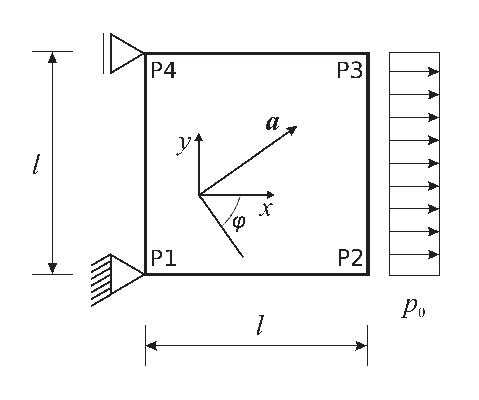
\includegraphics[scale=0.75]{M/figure/tenstest_model_mod.eps}
\end{center}
\caption{Tensile test. Model definition according to Kohlmeier \cite{Kohlmeier:2006}. Vector $\miu{a}{}{}$ defines the direction of anisotropy.}
\label{tens_transiso_model_2d}
\end{figure}

\subsubsection*{Initial and boundary conditions}

Initial conditions do not have to be given for the problem under consideration. The left-hand edge is fixed in horizontal direction. To avoid rigid body motions, the left lower corner node is fixed in both vertical and horizontal directions. A distributed tension load of $p_0=0.2\,$Mpa is applied at the right-hand edge. 

\subsubsection*{Material properties}

The material parameters are summarized in Tab.~\ref{matpar_transiso_tens}.

\begin{table}[!htb]
\centering
\begin{tabular}{lll}
\hline\hline\noalign{\smallskip}
Property & Value & Unit \\
\noalign{\smallskip}\hline\noalign{\smallskip}
Young's modulus $E_i$ & 561.12 & MPa \\
Young's modulus $E_a$ & 1311.83 & MPa \\
Poisson's ratio $\nu_i$ & 0.6032 & -- \\
Poisson's ratio $\nu_{ia}$ & 0.1838 & -- \\
shear modulus $G_a$ & 375.0 & MPa \\
\noalign{\smallskip}\hline\hline
\end{tabular}
\caption{Material parameters}
\label{matpar_transiso_tens}
\end{table}

\subsubsection*{Results}

The numerical results obtained with {\sl OpenGeoSys} are compared to values given in \cite{Kohlmeier:2006}. They include displacement coefficients of various corner nodes of the plate depending on the anisotropy direction, and show a good agreement (cf. Fig.~\ref{tens_transiso_test_2d}). 

\begin{figure}[!htb]
\begin{center}
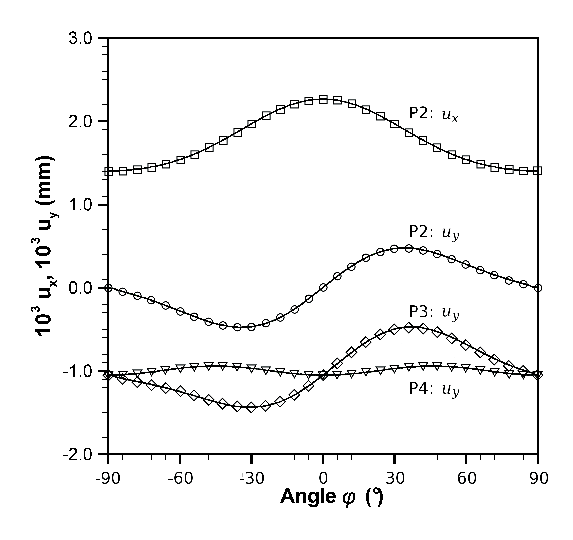
\includegraphics[scale=0.7]{M/figure/tenstest_results_OGS.eps}
\end{center}
\caption{Tensile test. {\sl OpenGeoSys} results (symbols) at length $l=10\,$mm and an edge load of $p_0=0.2\,$Mpa compared to the reference solution given by Schr\"oder \cite{Schroeder:1996} and Kohlmeier \cite{Kohlmeier:2006} (continuous lines).}
\label{tens_transiso_test_2d}
\end{figure}

\subsubsection*{Benchmark deposit}

\begin{tabular}{|l|l|l|}
  \hline
  Benchmark & Problem type & Path in benchmark deposit \\
  \hline
 \emph{m\_e\_transiso\_2D} & M & benchmarks\verb \M\ \\
  \hline
\end{tabular}

